%%%%%%%%%%%%%%%%%%%%%%%%%%%%%%%%%%%%%
% This is root file of the thesis. %
%%%%%%%%%%%%%%%%%%%%%%%%%%%%%%%%%%%%

%\documentclass[11pt,a4paper,oneside]{thesis}
\documentclass[11pt,a4paper]{thesis}
\usepackage{amssymb}
\usepackage{amsbsy}
\usepackage{amsmath}
\usepackage{hyperref}
\usepackage{algorithm}
\usepackage{pifont}% http://ctan.org/pkg/pifont
\newcommand{\xmark}{\ding{55}}%
\usepackage{amsthm} % This is only for theorem and proofs.
\usepackage{setspace}
\usepackage{listings}%code listing
\usepackage{xcolor}%commend colour
\usepackage{array}%tabular width
\usepackage{multirow}%
\usepackage{multicol}%
\usepackage{subfigure}%
\usepackage{courier}%inline code
\usepackage{fontspec}
\usepackage{minted}
\setmonofont{Courier New}
\definecolor{CPPLight}  {HTML} {686868}
\definecolor{CPPSteel}  {HTML} {888888}
\definecolor{CPPDark}   {HTML} {262626}
\definecolor{CPPBlue}   {HTML} {4172A3}
\definecolor{CPPBrown}  {HTML} {A07040}
\definecolor{CPPRed}    {HTML} {AD4D3A}
\definecolor{CPPViolet} {HTML} {7040A0}
\definecolor{CPPGray}  {HTML} {B8B8B8}
\definecolor{CPPGreen}  {HTML} {487818}%commends green
%\newfontfamily{\monaco}{Monaco}
%\lstset{basicstyle=\monaco}

\usepackage{ifpdf}
\ifpdf
\usepackage[pdftex]{graphicx}
\else
\usepackage{graphicx}
\fi
\usepackage{cite}
\title{Fuzzing Netlist}
\author{Shun Wan}


%%%%%%%%%%%%%%%%%%%%%%%%%%%%%%%%%%%%
% including page setting & fancyhdr.
\setlength{\textwidth}{500pt}
\addtolength{\hoffset}{-20pt}
\setlength{\textheight}{650pt}
\setlength{\headsep}{30pt}

% Set left margin - The default is 1 inch.
\setlength{\oddsidemargin}{2cm}
%\setlength{\evensidemargin}{0.63cm}

% Set width of the text - What is left will be the right margin.
\setlength{\textwidth}{15cm} %5.7in

% Set top margin - The default is 1 inch
\setlength{\topmargin}{-1.5cm}

% Set height of the header
\setlength{\headheight}{1.2cm}

% Set vertical distance between the header and the text
\setlength{\headsep}{1.2cm}

% Set height of the text
\setlength{\textheight}{23cm} %9in

% Set vertical distance between the text and the
% bottom of footer
\setlength{\footskip}{0.4cm}

% set belowcaptionskip.
\addtolength{\belowcaptionskip}{2ex}

\setlength{\parindent}{2em}
%\setlength{\parindent}{0pt}
%%%%%%%%%%%%%%%%%%%%%
\usepackage{fancyhdr}

\pagestyle{fancy}

\renewcommand{\chaptermark}[1]{\markright{\thechapter.\ #1}}
\renewcommand{\sectionmark}[1]{\markright{\thesection\ #1}}
\fancyhf{}
\fancyhead[LE,RO]{\bfseries\thepage}
\fancyhead[LO]{\bfseries\rightmark}
\fancyhead[RE]{\bfseries\leftmark}
\renewcommand{\headrulewidth}{0.5pt}
\renewcommand{\footrulewidth}{0pt}
\addtolength{\headheight}{0.5pt}
\fancypagestyle{plain}{
  \fancyhead[LE,RO]{\bfseries\thepage}
  \fancyhead[LO]{}
  \fancyhead[RE]{}
  \renewcommand{\headrulewidth}{0.5pt}
} 

\def\mystretch{1.5}

\newlength{\figX}
\newlength{\figY}
\newlength{\tmplen}

\newlength{\matFigX}
\newlength{\matFigY}

\setlength{\matFigX}{4.04in} \setlength{\matFigY}{3.04in}

\setlength{\parindent}{0pt}
\setlength{\parskip}{1ex}
\setlength{\parindent}{3em}
\sloppy

\hyphenation{another}

%%%%%%%%%%%%%%%%%%%%%%%%%%%%%%%%%%%
% The Beginning of a LaTeX document
\begin{document}

%%%%%%%%%%%%%%%%%%%%%%%%%%%%%%%%
% The Cover Page of PhD Thesis %
%%%%%%%%%%%%%%%%%%%%%%%%%%%%%%%%
\thispagestyle{empty}

\begin{center}
\null \vspace{\stretch{0.2}}
\renewcommand{\baselinestretch}{2}

\textsc{\huge{Fuzzing Netlist}}



\vspace{\stretch{1}}
\textsc{\large{Shun Wan}} \\

\vspace{\stretch{1}}

\vspace{\stretch{1}}
\textit{Supervised by}
\textsc{\large{Dr. John Wickerson}}\\
\vspace{\stretch{1}}

\vspace{\stretch{1}}
A Thesis submitted in fulfilment of requirements for the degree of \\
Master of Science\\
Future Power Network\\
of Imperial College London
\vspace{\stretch{1}}
%\centerline{\special{bmp:ic.bmp x=2cm}}
%\centerline{\hbox to 2cm{\epsfig{file=ic.eps,width=2cm,clip=}}}


\vspace{\stretch{0.1}}


Department of Electrical and Electronic Engineering\\
Imperial College London\\
\today

\end{center}




%%%%%%%%%%%%%
\frontmatter
\doublespace
\setlength{\tmplen}{\parskip}
\setlength{\parskip}{-1ex}
\renewcommand{\baselinestretch}{1.5}
\chapter{Abstract}
\renewcommand{\baselinestretch}{\mystretch}

%\setlength{\parindent}{2em}
Fuzz testing uses the random generalised data (inputs) to detect the bugs or code error in the software \cite{miller2007fuzz}.
% JW: It's not important to describe the history of fuzzing in the abstract. Only the most important parts should go into your abstract.
% JW: Citations go before the full-stop. So you should write, for example, "in 1988 \cite{miller2007fuzz}."
This thesis summarises 
% JW: Use present or future tense in the abstract, not past tense. So it should be "summarises".
the research project of fuzzing test in hardware synthesis, especially in netlists. Typically, the main application of fuzzing algorithm is used in software testing. Applying it to hardware synthesis software testing is a effective way to obtain the potential crashes or bugs in these synthesis tools. There are two main contribution of this project, the fuzz testing algorithm
% JW: algorithm
has been advanced and the tested. This project achieve the....
In addition, 
% JW: "the tested" ??
% JW: The abstract needs to be self-contained, so you can't end with "the following parts".

%The abstract is written here. This should concisely state the main aim of the work and the achievements.








\renewcommand{\baselinestretch}{1.5}
\chapter{Acknowledgement}
\markright{Acknowledgement}
\renewcommand{\baselinestretch}{\mystretch}
%\setlength{\parindent}{2em}
First, I would like to express my grateful thanks to my supervisor Dr.John Wickerson for his kind guidance through this academic year. His erudite knowledge and open-mind inspire me during this individual project and even future academic research life. More important, he taught me the critical and analytic thinking will benefit me all my life.I am grateful and fortunate to develop this MSc project under his supervision.

With the kind help of academic staff of Berkeley University, Alan, this project achieve. He sharing his brilliant idea and thoughts. The source code of SIS and some background resource are obtained. 
%JW: That's not a full sentence.

I would also like to thank my parents who support me through my life.












\tableofcontents
\listoffigures
\listoftables
\renewcommand{\baselinestretch}{\mystretch}
\renewcommand{\baselinestretch}{1}
\chapter{Abbreviations}
\markright{Abbreviations}

\begin{tabular}{rl}
  \vspace{0.1em} \textbf{DUT:} & Device Under Testing \\
  \vspace{0.1em} \textbf{DOS:} & Denial Of Service\\
  \vspace{0.1em} \textbf{HDL:} & Hardware Description Language\\
  \vspace{0.1em} \textbf{VHSIC:} & Very High Speed Integrated Circuit\\
  \vspace{0.1em} \textbf{VHDL:} & VHSIC Hardware Description Language\\
  \vspace{0.1em} \textbf{SQL:} & Structured Query Language\\
  \vspace{0.1em} \textbf{OSP:} & Open Source Project\\
  \vspace{0.1em} \textbf{GCC:} & GNU compiler collection\\
  \vspace{0.1em} \textbf{FDIV:} & Floating Point Division\\
  \vspace{0.1em} \textbf{LTS:} & Long Term Support\\
  \vspace{0.1em} \textbf{EDA:} & Electronic Design Automation\\
  \vspace{0.1em} \textbf{AIGs:} & And-Inverter Graphs\\
  \vspace{0.1em} \textbf{IDE:} &  Integrated Development Environment\\
  \vspace{0.1em} \textbf{OS:} & Operation System\\
\end{tabular}

\setlength{\parskip}{\tmplen}

%%%%%%%%%%%%
\mainmatter
\fancyhead[RE]{\emph{Chapter \thechapter}}
\renewcommand{\baselinestretch}{\mystretch}
% Use \input to include your chapters as illustrated below
\chapter{Introduction}
\renewcommand{\baselinestretch}{\mystretch}
\label{chap:Intro}
%\setlength{\parindent}{0pt}

\PARstart{F}{uzz} testing, also known fuzzing test, is a kind of software test technique that involves providing invalid, unexpected or random data as input to a compiler \cite{miller2007fuzz}. As a quality assurance technique, fuzz testing is efficient to find the coding errors and security loopholes in the compiler even in high level operating systems and networks. With large amount of random input data, the under tested device is attempt to crash or suffering memory overflow issue. If a vulnerability is detected in the software, the potential cause of the crash or error is also need to be identified. The identification is to located the error and comparing the influence with the error reference table. The ''fuzzer'' is defined to generate the large random inputs and identify the potential cause of the error or crash. Due to the acknowledge of the device under test (DUT)'s inside structure, the fuzzer can be categorised as white-box, grey-box and black box.

In conventional hardware design, the truth table and boolean expression need to be simplified manually and realised in real logical gate circuit. This process is cumbersome and error-prone. By working in a high abstract level which means only specific the logic function and involved the computer aided design (CAD) can greatly improve the design efficiency and reduce the number of design errors \cite{harris2015digital}. 
The modern hardware design and verification is heavily reliant on the HDL such as Verilog, SystemVerilog and VHSIC (Very High Speed Integrated Circuit) Hardware Description Language (VHDL). As a mainstream HDL, Verilog was standardised as IEEE 1364 in 2009 \cite{1620780} which occupied a large market share in industry and commercial application area. In 2009 the Verilog standard (IEEE 1364-2005) was merged with SystemVerilog standard and officially become a part of SystemVerilog. Since, a new standard was formed as IEEE 1364-2005. Comparing with VHDL, Verilog has more compact statements and more flexibility. As a consequence, the Verilog was chosen as the HDL in this project. The HDL code file needs to be transformed to a netlist by a hardware synthesis tool, for example VIVADO and ModelSim. The correctness of synthesis is the basis of the electronic production. It is important to design a test algorithm for the hardware synthesis tool.
% JW: But *why* is it important? It's crucial that you explain this to your readers. Why do hardware synthesisers need testing? What might happen if they have bugs?
\section{Motivation}
% JW: Aha, this is what I was missing earlier! Ok, the following subsection needs to come *much* earlier. The first thing you need to do in your report is convince your readers that you are solving an important problem. Once you have done this, *then* you can talk about your solution (which is fuzzing).
First of all, the high reliability of the synthesis tool is important to the synthesised circuit. Hoang M. et al have shown that most of the incorrect generations of netlist related to the Trojans in synthesis tool rather than invalid HDL code \cite{torjans}. Despite the development of self-verification, external testing is necessary. For instance, Intel's famous floating point division (FDIV) bug in the Pentium processor was discovered by Prof. Thomas R. Nicely at Lynchburg College \cite{Intelbug}. Due to this bug, the processor may process a wrong result when dividing a number. The incorrect calculated result occurring probability is 1 in 9 billion FDIV with random parameters. As estimated, recalling the defect processors and replacement them costed Intel company approaching 475 million dollars. Lack of third-party verification and testing may cause the synthesis tool become even more error-prone.

Secondly, the existing testing tool has several limitations. The coverage of the test is narrow. For the existing synthesis tool testing software, VlogHammer's generations are concentrated on combinatorial circuit with small number of ports and terminals. Large scale of fuzz input may more effective than original method. 

In addition, this project has comprehensive research foreground 
% JW: What does "comprehensive research foreground" mean?
and potential value.
% JW: "potential value" is too vague -- be more specific about what the value is.
Big data analytic offers effective statistical power and can be used in predictive analytic and user behaviour analytic. In future, the investigation of performance of the fuzzer and the detected vulnerabilities identification can be matured by big data analytic. This cross subject analysis may shedding light on what feature of the fuzz testing algorithm need to be developed related to bug-hunting ability.
\section{Fuzzing in hardware synthesis}
In 1989, the fuzz testing algorithm was initially proposed by Barton Miller at University of Wisconsin \cite{miller2007fuzz}. He designed a fuzzer to automatically generate random file and command lines to test the utility of an Unix-based application. The debugging tool to identify the cause of crash was also provided by him. As presented in his paper \cite{miller1990empirical}, 25-33\% of the utility programs on different version of UNIX system were crashed during the fuzz testing. Above results shows that this testing algorithm is effective to finding the bugs existed in the DUT. At present, the definition of term fuzz testing is not limited in the command-line utilities.
Although the weakness of the fuzz testing algorithm is the bug-finding pertinence is not robust. 
% JW: What do you mean by "bug-finding pertinence"?
With the simple design structure, high practicability and capability, it has impressive cost-efficient ratio in debugging area to discover severe overlooked defects. Different from other testing algorithm and method, it has advantage that does not need oracle for test results. For software testing, the main application of this testing algorithm is to discover the vulnerabilities such as buffer overflow,
denial of service (DOS), cross-site scripting and structured query language (SQL) injection\cite{Yang:2011:FUB:1993316.1993532}. 

Based on above discussion, the purpose of this project is to apply this fuzz testing algorithm in hardware synthesis tool. With the trend of open source project(OPS), this project is focusing on low-level open-source hardware synthesis software for example, ABC and SIS. The random generated HDL files will be entered to a hardware synthesis software by a bash shell program. Inspired by Xuejun Yang and his colleagues designed Csmith \cite{Yang:2011:FUB:1993316.1993532}, the basic block diagram of this project shows in Fig \ref{Fig:Block diagram}. On the left-hand side, GNC compiler collection (GCC) and Microsoft's Visual studio (MSV) are C compilers and on the right-hand side, ABC and SIS are hardware synthesis software. Different from the software fuzz testing, the input netlist file can directly comparing with the output of the hardware synthesis tool. Because these two files are in same format and easy to do the function test. Comparing the synthesised netlist with its original input circuit, if these two circuits are not equivalent, it indicates that might be a bug existing in the tested tool. 
% JW: The figure is nicely drawn, but it doesn't actually reflect your toolflow. On the left-hand side you're comparing the outputs of *two different* C compilers. But in your toolflow, you only need *one* hardware synthesiser, because you compare the *input* of the tool against its *output*. You're not comparing the output of ABC against the output of SIS, which is what your diagram shows.

\begin{figure}[htb]
\centering
\begin{minipage}[htb]{1\textwidth}
\centering
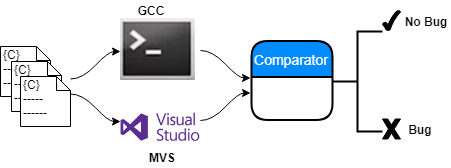
\includegraphics[width=8cm]{MScThesisTemplate/Figs/1.png}
\end{minipage}
\begin{minipage}[htb]{1\textwidth}
\centering
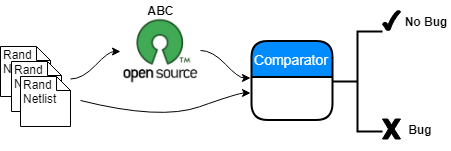
\includegraphics[width=8cm]{MScThesisTemplate/Figs/2.png}
\end{minipage}
\caption{Block diagram}
\label{Fig:Block diagram}
\end{figure}

\section{Project Contribution}
The main contributions of this project are:
\begin{itemize}
    \item Applying the fuzz testing algorithm in open-source hardware synthesis tool testing field. The fuzz testing method's state of art was advanced and extended. The random generated file has better coverage and more esoteric comparing to typical Verilog code file generated by existing testing tool.
    \item Detected bugs and crash issue were analysed through qualitative and quantitative. Not only benefits the debug and version updating for the hardware synthesis tool, but also worthy in big data research in bug-hunting. 
    \item With further polishing, the designed testing tool can be promoted as a distributed Linux software in a collaborative public manner.
\end{itemize}

\section{Thesis Outline}
This thesis is divided into 6 chapters to illustrate the design and implementation of the fuzzing netlist. Following the first introduction, the background chapter 2 will demonstrate the theory applied in this project with the literature review. Chapter 3 discuss the project plan including the objectives and strategy for evaluating the project. In Chapter 4 the detail implementation of combinational and sequential testing circuit with high-level coding language. The bash shell program with error detection will also be presented. The result and future improvement of designed the fuzzer and toolflow will be depicted and evaluated in Chapter 5. In the final chapter 6, it conclude the impact of the project and future work. 
\chapter{Background}
\renewcommand{\baselinestretch}{\mystretch}
\label{chap:Back}
%\setlength{\parindent}{0pt}
\PARstart{B}{ack} ground theory, related research and existing tool will be provided in this chapter with detailed illustration. The first section 2.1 will further describe the fuzz testing model selection foundation. The design trade-off was considered between three mainstream model type: black box, grey box and white box. Following section introduce the tested hardware synthesis tool: Berkeley design ABC with its highlights and innovative algorithms. In the final section, the investigation and evaluation of existing fuzz testing tool in hardware synthesis: VlogHammer will be presented.
\section{Fuzz testing and model selection}
As mentioned before, the fuzz testing was pioneered by Dr.Barton Miller. Through 20 years development, it has been matured in software validation and security testing area. Microsoft's Springfield Project applied fuzzing as a service. OSS-Fuzz Continue from Google provide fuzz testing for open-source projects. According to the acknowledge degree of inside structure or code of DUT, the fuzz testing model can be ranked as white-box, grey-box and black-box.
\subsection{Black-box fuzzing}
The Black-box fuzzing is regarded as a random testing method which only considers the correctness of the output results or function. It based on the pre-defined specified or required input, called seeded input \cite{nidhra2012black}. The inside structure and operation principle are not concerned in this kind of test model.Fig \ref{fig:balckbox} shows the construction of the black-box model. 
\begin{figure}[htbp]
    \centering
    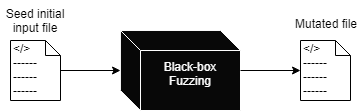
\includegraphics[scale=0.8]{MScThesisTemplate/Figs/balckbox.png}
    \caption{Black-box fuzzing}
    \label{fig:balckbox}
\end{figure}

Mutation is the important characteristic of black box fuzzing. With a valid initial seed, the output of test generator can be randomly mutates to other test-generation heuristics \cite{bounimova2013billions}. The DUT's bugs or vulnerabilities are expected to be evoked by the randomly generalised inputs. Black-box testing is a cost-effective method in bug finding. According to prescription of multinational technology company like Microsoft \cite{bounimova2013billions}, black-box fuzzing is a compulsory procedure of every newly designed device or programmed software. It is knows as "Security Development Lifecycle" \cite{howard2006security} in Microsoft product manual. However, the disadvantage of the black-box fuzzing is relative low code coverage and bug missing. The following short program shows that the probability of triggering the conditional branch \texttt{then} is $1/2^{32}$. Because \texttt{int} type is a 32-bit long parameter and only one corresponding number \texttt{2019} can induce the error issue.

\begin{lstlisting}[float=htb,
        label=lstcode,
        language=C++,
        basicstyle={\ttfamily},
        keywordstyle=\color{blue}, 
        commentstyle=\color{CPPGreen},
        escapeinside=``,
        %breaklines,
       xleftmargin=2em,xrightmargin=2em, aboveskip=1em,
        tabsize=4]
int fuzz(int x){
    int y = x + 1;
    if (y == 2019) 
        abort();//Bug location
    return 0;
}
\end{lstlisting}

\subsubsection{Csmith}
Csmith is a typical implementation of blaxk-box fuzzing. As Xuejun Yang, Yang Chen et al, mentioned in their paper \cite{Yang:2011:FUB:1993316.1993532} they designed Csmith as a "randomised test-case generation tool". The generated C program by Csmith involved most kinds of C expressions and statements defined in C99 standard. Other commonly used features in C language such as control flow (\texttt{if/else},\texttt{for} loop, \texttt{break}), variable definition (\texttt{int},\texttt{char}), operation (arithmetic, logical and bitwise) are also covered in Csmith. The structure of the Csmith shows in the Fig. \ref{Fig:csmith}. The test harness has been passed to three different compilers to execute it. Comparison among the three compilers, the minority result indicates that it has large probability containing bugs or vulnerabilities. 

Avoid inadequacies for the compilers, each generated program by Csmith has a unique interpretation. Csmith's C program generation follows top-down architecture. The global environment of Csmith describe the highest level definitions. The local environment defines three information: current call chain, objects and all in-scope pointers \cite{Yang:2011:FUB:1993316.1993532}. Guided by probability table, the Csmith construct the c code file step by step from basic \texttt{main} to branch function and sub-objects. The researchers spent three years to find serves, previous unknown bugs in mainstream C compilers such as GCC, LLVM and other commercial tools. End till the publish of their paper, the number of detected unknown bugs is 325 and has been reported to the compiler developer. These bugs and vulnerabilities including compiler crash and return wrong compiling output results \cite{klees2018evaluating}. The quantitative analysis of Csmith shows that the code coverage of Csmith is high in line(75.58\%) and function(82.41\%), but low in branch(46.26\%). The cumulative distinct crash error of Csmith is 86 which in significantly.

Csmith proves that black-box fuzzing is a worth considering model in hardware synthesis tool testing. Because the impressive effectiveness of bug finding, detected 325 unknown bugs in short 3 years. The design structure is easy to understand and implement.

\begin{figure}[htbp]
\centering
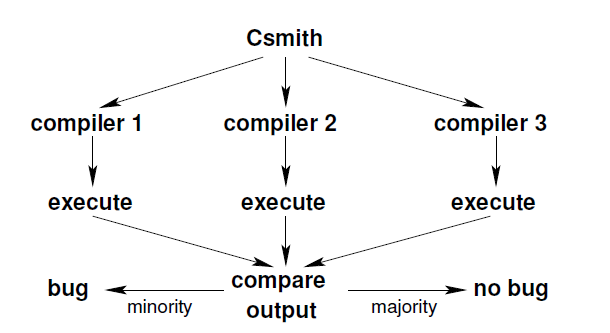
\includegraphics[scale=0.6]{MScThesisTemplate/Figs/Csmith.PNG}
\caption{Csmith architecture \cite{Yang:2011:FUB:1993316.1993532}}
\label{Fig:csmith}
\end{figure}

\subsection{White-box fuzzing}
White-box fuzzing is an alternative fuzz testing method. With the development of systematic dynamic test generation \cite{godefroid2005dart}, the white-box fuzzing has been extended from unit-level to integration and system level. The white-box fuzzer will dynamically operate the symbolic executed input until all feasible path of the DUT has been swept through. Testing structure of the white-box fuzzing shapes a "Tree" which is provided in Fig.\ref{fig:whitebox}. Using above program in \ref{lstcode} as example, the initial seed value of input \texttt{x} is \texttt{1} and \texttt{y = x + 1} which will assign \texttt{2} to \texttt{y}. The path constrain \texttt{2} $\neq$ \texttt{2019} yields the execution of conditional branch \texttt{else}. Finishing execution of one conditional branch under such constraint, the next generated input would be \texttt{x = 2018} to allow the execution of the other conditional branch. The input format or other specification do not need to know. Moreover, each individual path of the DUT and internal perspective of the DUT will be egoistic tested. This guarantee the high code coverage of white-box fuzzing. \cite{functest}

Comparing to black-box fuzzing, white-box fuzzing has advantage in full path thorough testing. The testing processes are traceable and easy to automate. In practice, the large scale of execution path of DUT can not be available to be tested. The large number of path can not be precisely within a reasonable time. Besides, white-box fuzzing increase the complexity to testing and reduce the universality. Therefore, the white-box fuzzer might be closely connected with the specific implementation of the DUT. Rewriting the output generated by designed fuzzer may lead assumption failure or occur unnecessary error \cite{nidhra2012black}\cite{bounimova2013billions}. Moreover, white-box fuzzing cost too much computational resource in dynamic symbolic execution. 
\begin{figure}[htb]
    \centering
    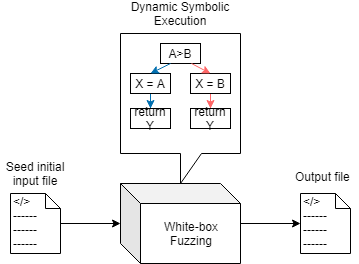
\includegraphics[scale=0.8]{MScThesisTemplate/Figs/whitebox.png}
    \caption{White-box fuzzing}
    \label{fig:whitebox}
\end{figure}
\subsubsection{SAGE}
In the published paper by Ella Bounimova, Patrice Godefroid and David Molnar \cite{bounimova2013billions}, they proposed an constraint-based white-box fuzzer SAGE. The developers aim to generate large numbers of instruction and statements in single symbolic execution. Thus, the generational search strategy of the SAGE was creative and innovative. The first step of symbolic execution will create a path constraint. As they described in their paper \cite{bounimova2013billions}, the rest of the constraints in this path will be solved by a constrain solver and ''placed in a conjunction with the prefix of the path constraint leading to it''. The static result shows that single execution can generate 25,598 full path constraints.

The structure of shows in Fig \ref{Fig:sage}. An initial input would be passed to SAGE to run the program test. If the program crashes, it means that this initial input may trigger a bug. If not, the SAGE will symbolically execute the program with that input and generate the required path constraints. When all the contraint in that path have been solved by the constraints solver, the satisfied constraints would be mapped into \texttt{N} different input to improve the instruction coverage. \texttt{N} constrains would be ranked in terms of the ability of discovering new instructions. The next symbolic execution of SAGE will adopt the highest mark input as its input \cite{bounimova2013billions}.

The result of SAGE show that the SAGE fuzzer can find around 50 unique bugs in 23 days of running it on 200 programs. Comparing with the bug hunting ability of black-box model(352 bugs in three year's testing), the efficiency have been greatly improved. It proves the advantage of white-box in high code coverage and full path through testing. However, the implementation of SAGE used the dynamic systematic generation execution. The structure diagram of SAGE (Fig \ref{Fig:sage}) is much more complicated than the black-box Csmith(Fig \ref{Fig:csmith}). 
\begin{figure}[htb]
\centering
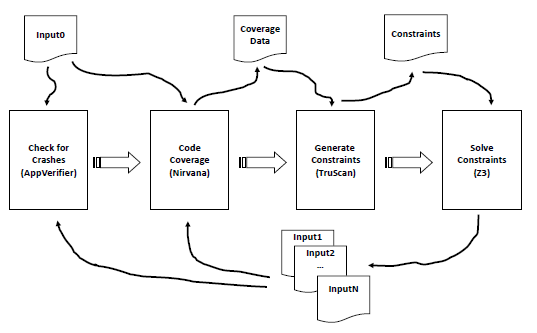
\includegraphics[scale=0.8]{MScThesisTemplate/Figs/sage.PNG}
\caption{SAGE architecture\cite{bounimova2013billions}}
\label{Fig:sage}
\end{figure}

\subsection{Tradeoff: Grey-box fuzzing}
Leveraging the pros and cons of black-box fuzzing and white-box fuzzing, this project decided to use the intermediate model: grey-box fuzzing model. Grey-box fuzzing integrate the features of black-box and white-box. It partly know the inside structure, code and algorithm of DUT but the test aim is correctness of output results based. It is beneficial in the hardware synthesis tool testing. Because the input file of a hardware synthesis tool require a specific format and the input HDL file should be synthesizable. For example, if the generated HDL file is a test-bench, it indeed a valid input file of the hardware synthesis tool but the synthesis tool can not yield a synthesised netlist. In addition, the output netlist circuit of the DUT not only expected to correctly execution but also expected to be synthesised in a optimised way. For instance, the \cite{havrikov2017efficient} %Need an example.
In addition,  
The detail part of this projects fuzzer will be presented in the methodology section of chapter 3.

\section{Hardware synthesis: Berkeley designed ABC}
ABC is a powerful synthesis and formal verification tool in hardware designs. It was developed by Robert Brayton and Alan Mishchenko in University of California, Berkeley. Since 2005, ABC has been gaining momentum and attention to be a ''public-domain'' tool in hardware logical synthesis and verification \cite{ABC}. In this project, ABC was used as a synthesis tool. As a result, the verification function of ABC was neglected. 
\subsection{Selection motivation}
The first reasons of selecting ABC as a DUT is that ABC occupies a dominant position in academic research. The user of ABC are University of Colorado (Boulder), Cornell University and University of California (Berkeley). If a bug or Vulnerability was found in the ABC, it is beneficial for the academic staff to avoid wrong scientific research. 

Secondly, the open-source feature of ABC is a huge merit. As a open-source tool of Electronic Design Automation(EDA), ABC is source code can be forked from Github \url{https://github.com/berkeley-abc/abc}. The open source mode can improve the software's reliability due to the contribution of thousands of independent programmers in software testing and bugs fixing.\cite{laurent2004understanding} With the source code of the ABC, the design of the fuzz testing software could use the grey-box fuzzing model. As discussed in above section, no doubt that the programmed testing tool will be more efficient and pertinence. Besides, the access of viewing and modifying source code of ABC allow us to inject bugs to ABC in future analysis.

The third reason of select ABC is its high efficiency. The synthesis method of ABC has switched from multi-level valued to binary And-Inverter Graphs (AIGs). Comparing to its predecessor SIS (developed by research group of UC Berkeley in 1987-1991\cite{ABC}), it saves the runtime and memory space. The scalability of ABC has increased due to the saving in above two aspects.

In addition, ABC attached equivalence checker provided a efficient way in final comparison stage of this project. The equivalence checker of ABC can handle both combinatioal and sequential circuit based on SAT sweeping \cite{satsweep,kuehlmann2001circuit}. Two circuits will be transformed into an equivalence checking miter which is consisted of EXOR gates and OR gates. 
The inputs of the original circuit will be transmitted to EXOR gates and ORed to yield a output of the miter. This equivalence checker has been awarded to out of three categories at hardware model checking competition at CAV 2008. It certified that the checking result of the equivalence is reliable.

\subsection{Highlights and commands}%这一部分还需要大改
Hardware synthesis tool is expected to convert a high-level HDL into an optimised gate-level representation (Netlist). The transformation need to satisfy some criteria such as optimise the gate number, logic level and node number. ABC combines scalable logic optimization based on AIG , optimal-delay DAG-based technology mapping for look-up tables and standard cells, and innovative algorithms for sequential synthesis and verification \cite{ABC}.\\
\textbf{Multiple in-out parse:}\\
\textbf{And-Inverter Graphs:}


The following tabale shows some circuit optimisation instruction involved in this project.
\begin{table}[!htbp]
    \centering
    \begin{tabular}{c|c|m{8cm}}
        \hline
       Command type & Command name & Function\\
        \hline
     \multirow{3}{*}{Synthesis}&\textbf{\texttt{balance}} & Assumes that the input is an AIG and creates an equivalent AIG having the minimum delay, measured using logic levels of two-input AND-gates. The inverters do not count towards the number of logic levels. The resulting AIG is derived by algebraic balancing of the multi-input AND-gates contained in the original AIG. The balancing is applied in the topological order and selects the minimum delay tree-decomposition of each multi-input AND-gate. Balancing takes into account the arrival times of primary inputs, which can be represented in BLIF.\\
     \cline{2-3}
     & \textbf{\texttt{strash}}&Transforms the current network into an AIG by one-level structural hashing. The resulting AIG is a logic network composed of two-input AND gates and inverters represented as complemented attributes on the edges. Structural hashing is a purely combinational transformation, which does not modify the number and positions of latches.\\
     \cline{2-3}
     & \textbf{\texttt{cycle}}&Simulates the sequential network with random input and updates its current state.\\
     \hline
     \multirow{2}{*}{Read}&\textbf{\texttt{read\_verilog}}&Parses the input file in a very limited subset of structural Verilog, which includes all the keywords and directives needed for reading IWLS 2002 Benchmarks and  IWLS 2005 Benchmarks. Before reading the latter, make sure the Cadence library is loaded into ABC using command \texttt{read\_library cadence.genlib}. When the library is loaded, use command \texttt{r –m <file.v>}\\
     \cline{2-3}
     & \textbf{\texttt{read\_aiger}} & Reads the combinational AIG in binary AIGER format developed by Armin Biere. This format is very compact and leads to a substantial reduction in the reading/writing times.\\
     \hline
     \multirow{2}{*}{Write}&\textbf{\texttt{write\_verilog}}& Outputs the network using technology-independent Verilog.\\
     \cline{2-3}
     & \textbf{\texttt{write\_verilog}}& Outputs the network using technology-independent Verilog.\\
     \hline
     
\end{tabular}

    \caption{Main commands related in this project\cite{manual2006quick}}
    \label{tab:my_label}
\end{table}



\section{Existing bug-hunting tool in hardware synthesis}
VlogHammer is a current existing regression Verilog test software to verify the circuit correctness of the Verilog \cite{wolf2016yosys}. As a powerful fuzzer VlogHammer can generate different types of combinational logic circuit in Verilog. The algorithm used by VlogHammer is based on divide-and-conquer.

\section{Related work}
\chapter{Project Design}
\renewcommand{\baselinestretch}{\mystretch}
\label{chap:ProDes}
\PARstart{T}{his} chapter illustrate the design process of this project. The first section 3.1 is divided into 2 subsection 3.1.1 and 3.1.2 to explains the core objectives and extensive objective this project. Next, methodology section 3.2 explains the algorithm design in flow chart and how to construct the developing environment. The final section discuss how to evaluate the result and performance of the designed fuzzer.
\section{Objectives}
\subsection{Core}
The core objective of this project is to write a program to generate simple combinational logic circuits (no clock signal) without sequential elements (flip-flop, register, ROM). A LINUX shell program need to be programmed to input the fuzzing netlist file to ABC.
\subsection{Extension}
The extension objective is constructing more complex circuit (not guaranteed to be supported by ABC). The generated circuit will be re-synthesized using the circuit folding method. Using sequential (Synchronous, Asynchronous, more than one clock signal) flip-flop, register, adder, mux and other logical elements. The input/output can be realized in tri-state. It indicates that the output port was allowed to yield high impedance state (z) and unknown state (x), in addition to the 1 and 0 logic states. 
\section{Methodology}
To achieve the aims and objective of this project, the research would be initially conducted on theoretical analysis. Understanding the basic principle of random variable generation and rules of Verilog file. To be specific, the first step is to analyze the synthesis principle of netlist file. For example, read the design specification from file and manual. Secondly, the tested hardware synthesis tool needs to be modified to accepted thousands of random inputs and output the results. The test target ABC is an open source software and its code can be modified by using C language compiler. The linux system is an effective environment to compile an open source software. As a consequence, the development of this fuzzing test will be implemented on Linux. Refer to the existing fuzzer, the fuzzer may also be compiled in C language by GNC compiler collection (GCC). For the extended objectives, the circuit optimization method is also required.

The practical implementation will be conducted on the
\section{Evaluation strategy}
The result will be evaluated in two aspect: qualities and quantities.

\begin{equation}
       \sum_{i=1}^{x} 
       \begin{pmatrix}
       n\\
       i\\
       \end{pmatrix}
       \theta^{i}(1-\theta)^{n-i}\ge\alpha
\end{equation}


\chapter{Project Implementation}
\renewcommand{\baselinestretch}{\mystretch}
\label{chap:Fuzzer}
\PARstart{T}{he} algorithm of randomly generating program is the core part of this fuzzer and could be adapted to the generation of the random netlists. In this project, the hardware description language Verilog is the design specification file of the random netlist. Verilog is traditionally used by hardware synthesis software to represent logic networks (logic-level hierarchical circuit in textual form). A standard \cite{1620780} presented by IEEE described the specific definition of Verilog, the circuit was regarded as a directed graph of combinational logic nodes and sequential logic elements. Models, Logical gates and Latches were main components of a Verilog file.
\section{Developing environment and tools}
As compiling based project, the first step is to decide the developing environment. For the DUT: Berkeley designed ABC and existing testing tool VlogHammer, these are all Linux software. Developing this project in a open source way can gather more people's brilliant idea and intelligence. The \texttt{Readme.txt} on Github of ABC shows that current version of ABC has been tested stable on current Linux distribution version in 32-bit and 64-bit. Considering above factors, this project was developed on Ubuntu 18.04.3 LTS.

Compile language of this project is selected as C++ due to its Object-oriented feature. As a popular  integrated development environment (IDE) on Linux  Visual Code on Linux system 
\section{Toolflow}
The designed \cite{fujita2018automatic} and \cite{godefroid2007random}.The developing environment is based on Linux Ubuntu 18 OS
\chapter{Result and Evaluation}
\renewcommand{\baselinestretch}{\mystretch}
\label{chap:Result}
\PARstart{O}{btained}result and data form fuzz testing will be displayed in this chapter with analysis and evaluation.
\chapter{Conclusion}
\renewcommand{\baselinestretch}{\mystretch}
\label{chap:Con}
\PARstart{I}{n} conclusion, this thesis

%%%%%%%%%%%%%%%%%%%%%%
% The reference list.%
%%%%%%%%%%%%%%%%%%%%%%

\renewcommand{\baselinestretch}{1}

% Note: put the bib style and bib file you use here.
\bibliographystyle{IEEEtran}
\bibliography{IEEEabrv,references}

%%%%%%%%%%%%%%%%%%%%%%%%%%%%%
% The end of reference list.%
%%%%%%%%%%%%%%%%%%%%%%%%%%%%% 
\fancyhead[RE]{\emph{References}}

\appendix
\renewcommand{\baselinestretch}{1.5}
\chapter{Appendix Title}
\label{App:Poly}

\newtheorem{Theorem}{Theorem}

\begin{Theorem}
It is sometimes desirable to place material in an appendix such as this. If you don't have any such material, then the appendix is of course optional. Many people manage without one.
\end{Theorem}
\begin{proof}
This is the proof.
\end{proof}
\renewcommand{\baselinestretch}{1.5}
\chapter{\texttt{ABC} visualisation}
\label{App:abc}
\begin{figure}[htbp]
    \centering
    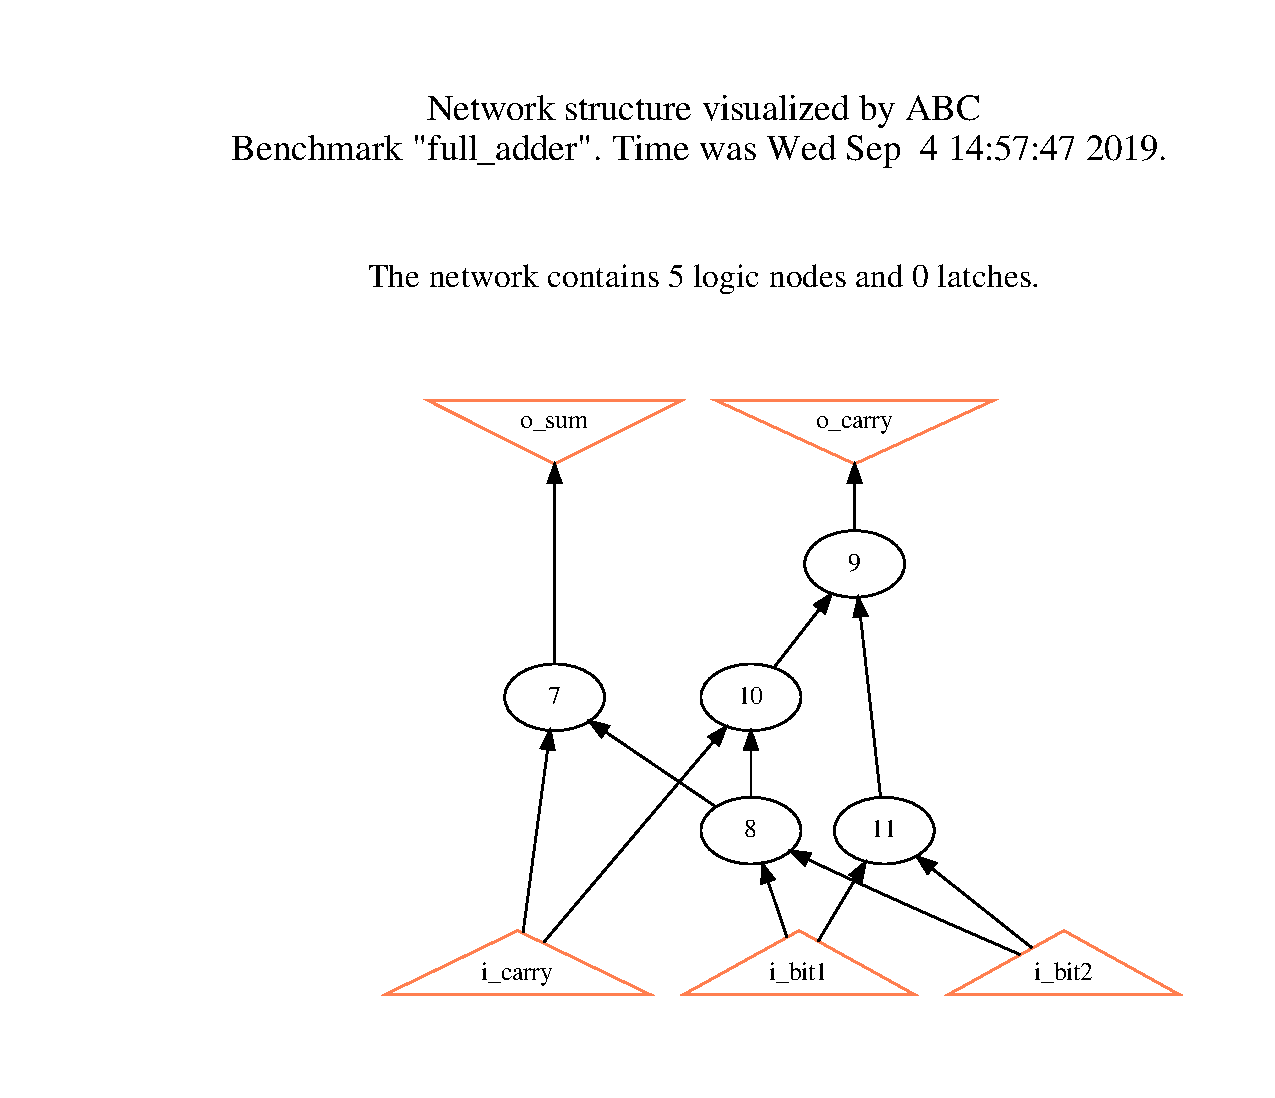
\includegraphics[width=15cm]{MScThesisTemplate/Figs/renode.pdf}
    \caption{\footnotesize renode}
\end{figure}
\begin{figure}[htbp]
    \centering
    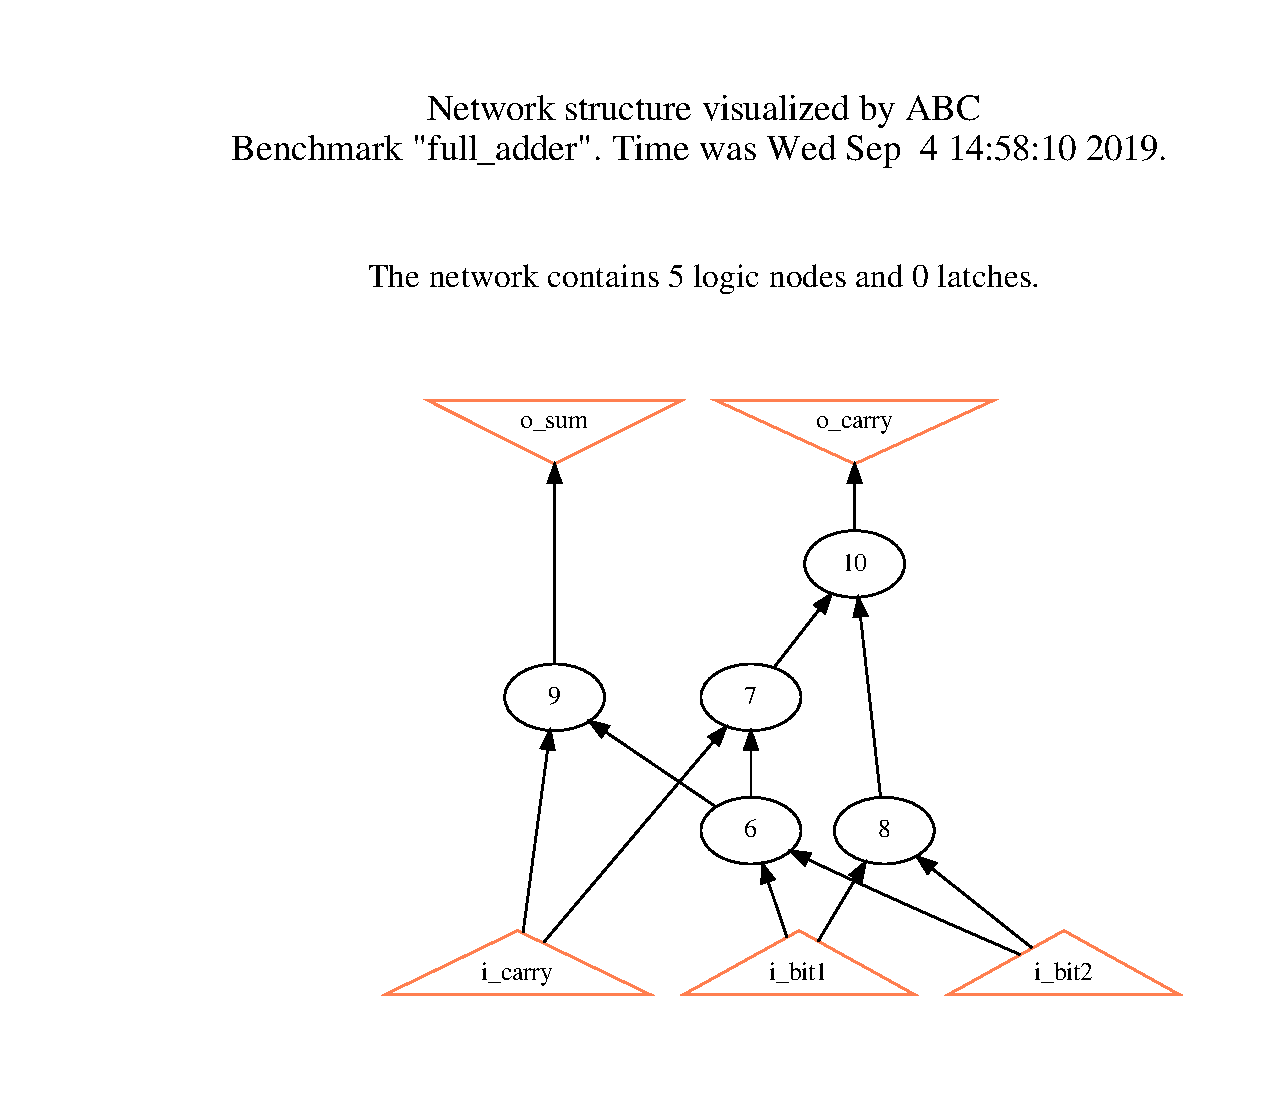
\includegraphics[width=15cm]{MScThesisTemplate/Figs/cleanup.pdf}
    \caption{\footnotesize cleanup}
\end{figure}
\begin{figure}[htbp]
    \centering
    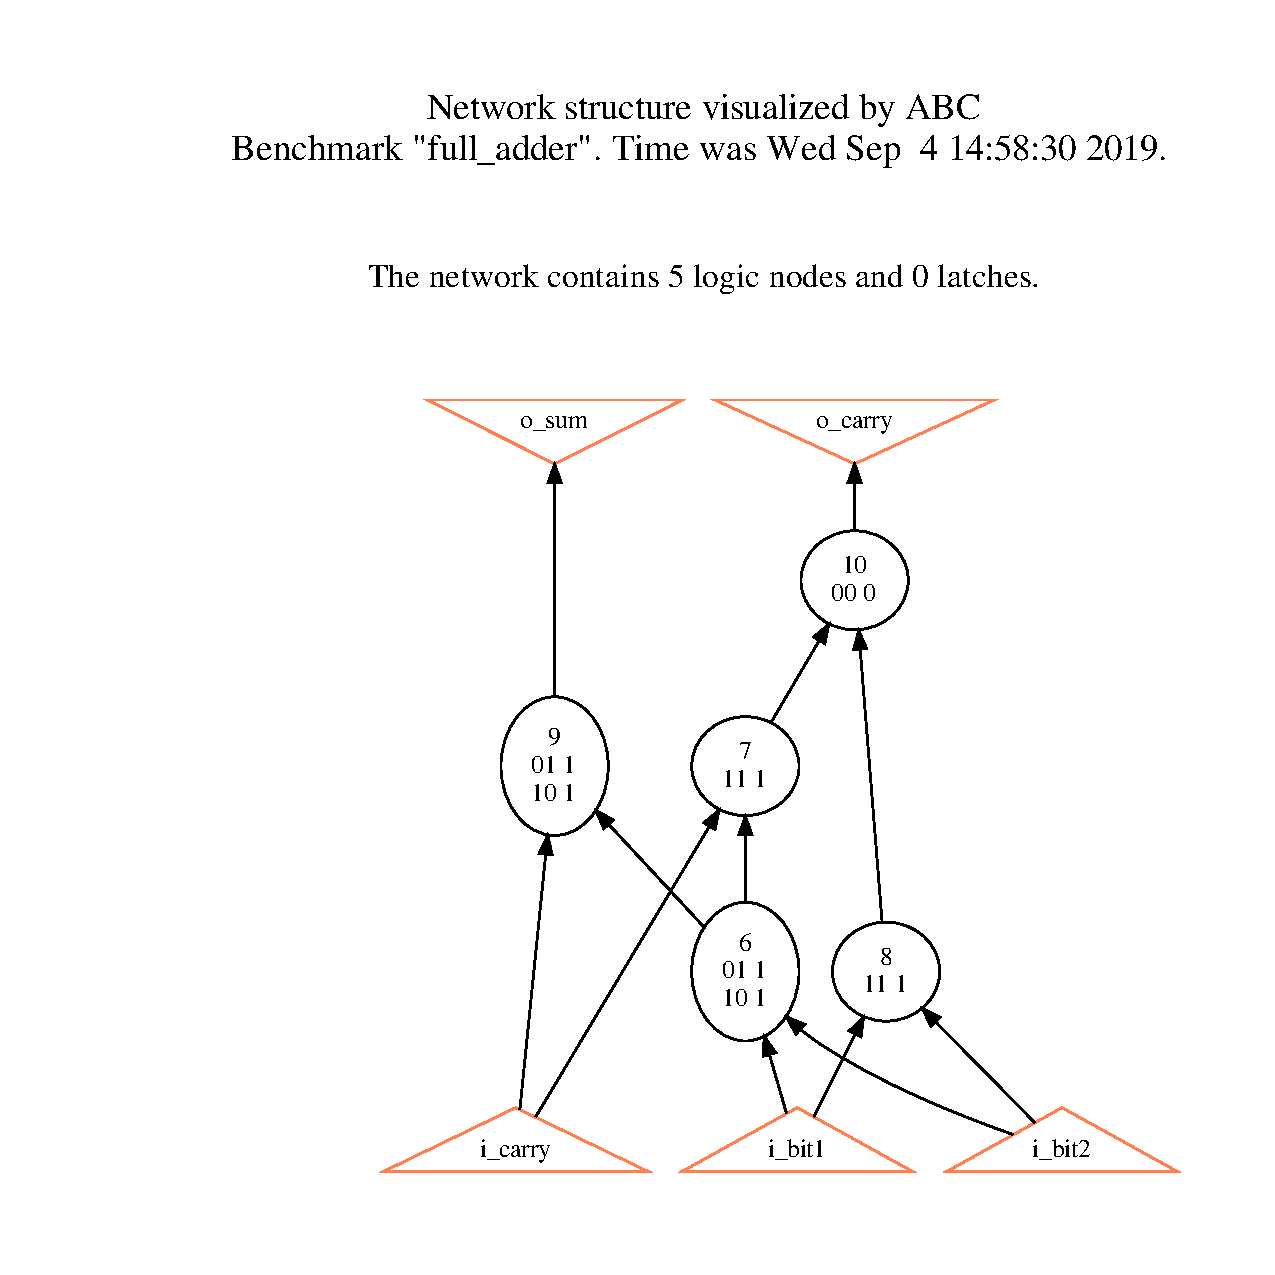
\includegraphics[width=15cm]{MScThesisTemplate/Figs/sweep.pdf}
    \caption{\footnotesize sweep}
\end{figure}
\begin{figure}[htbp]
    \centering
    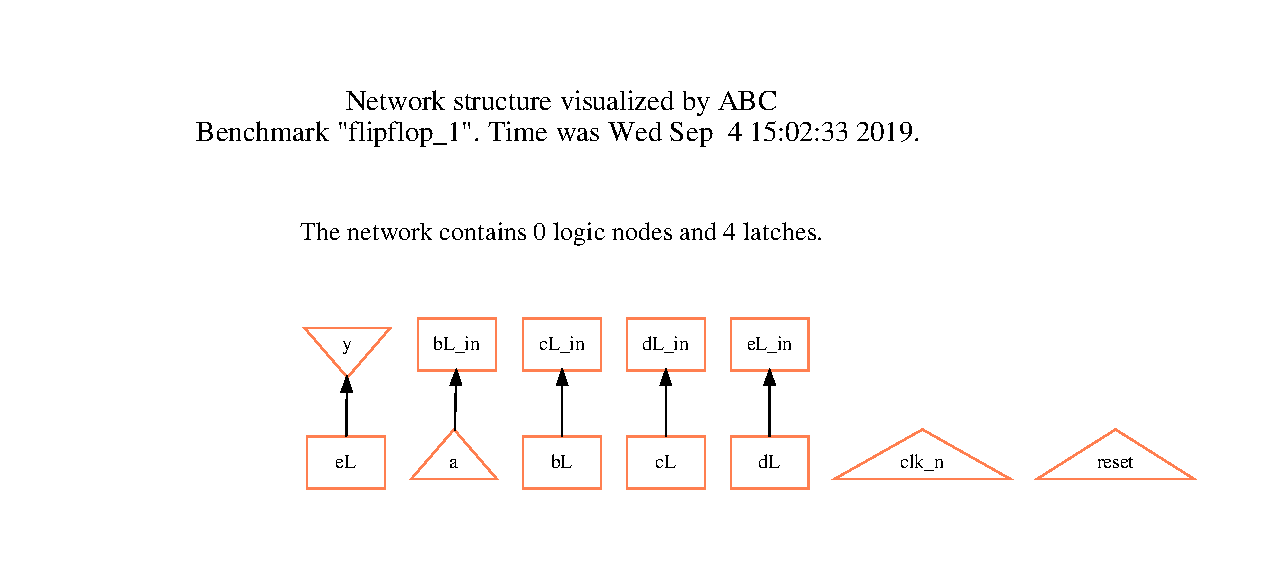
\includegraphics[width=15cm]{MScThesisTemplate/Figs/cycle.pdf}
    \caption{\footnotesize cycle}
\end{figure}
\begin{figure}[htbp]
    \centering
    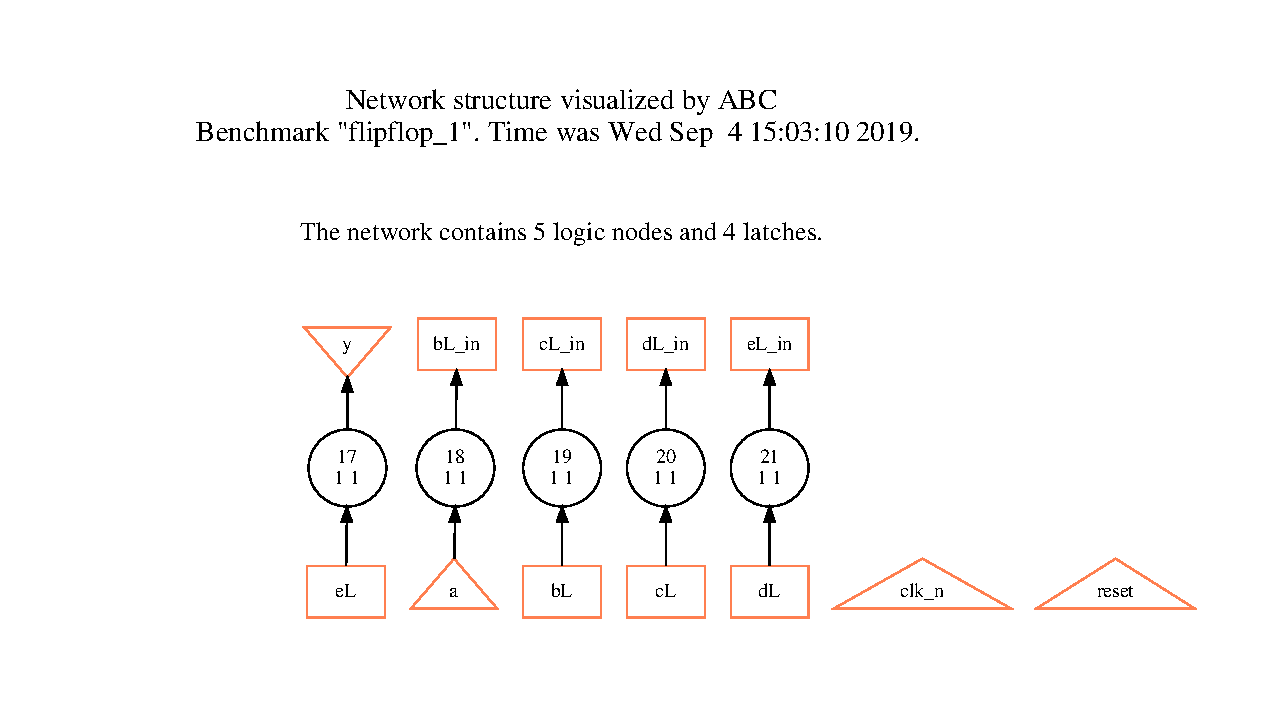
\includegraphics[width=15cm]{MScThesisTemplate/Figs/retime.pdf}
    \caption{\footnotesize retime}
\end{figure}
\begin{figure}[htbp]
    \centering
    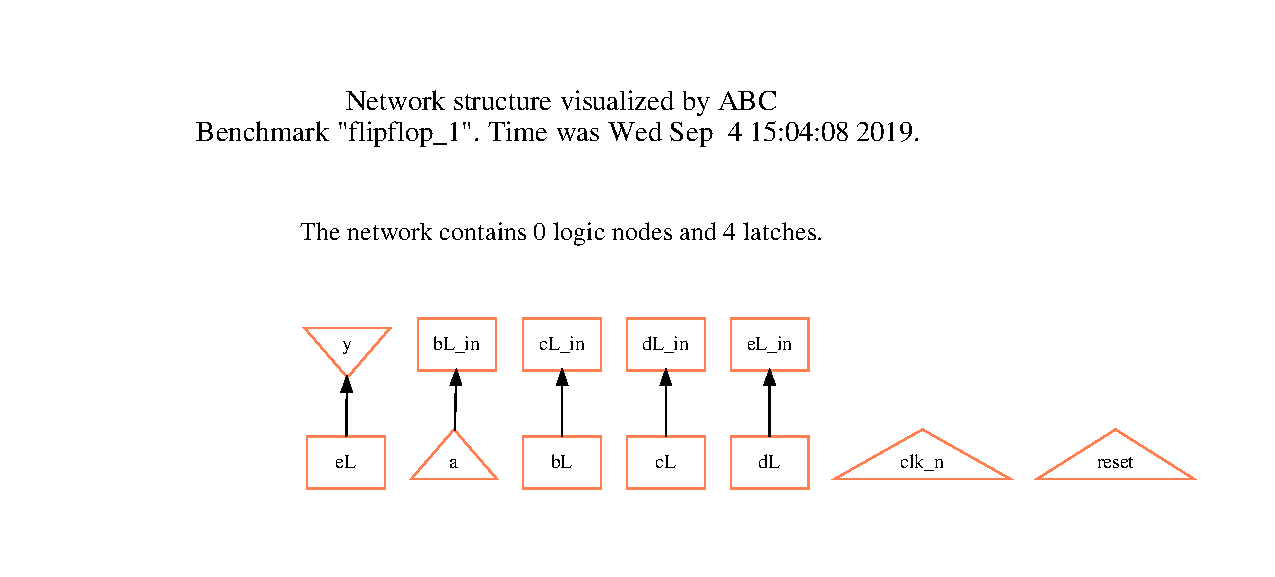
\includegraphics[width=15cm]{MScThesisTemplate/Figs/scleanup.pdf}
    \caption{\footnotesize scleanup}
\end{figure}
\begin{figure}[htbp]
    \centering
    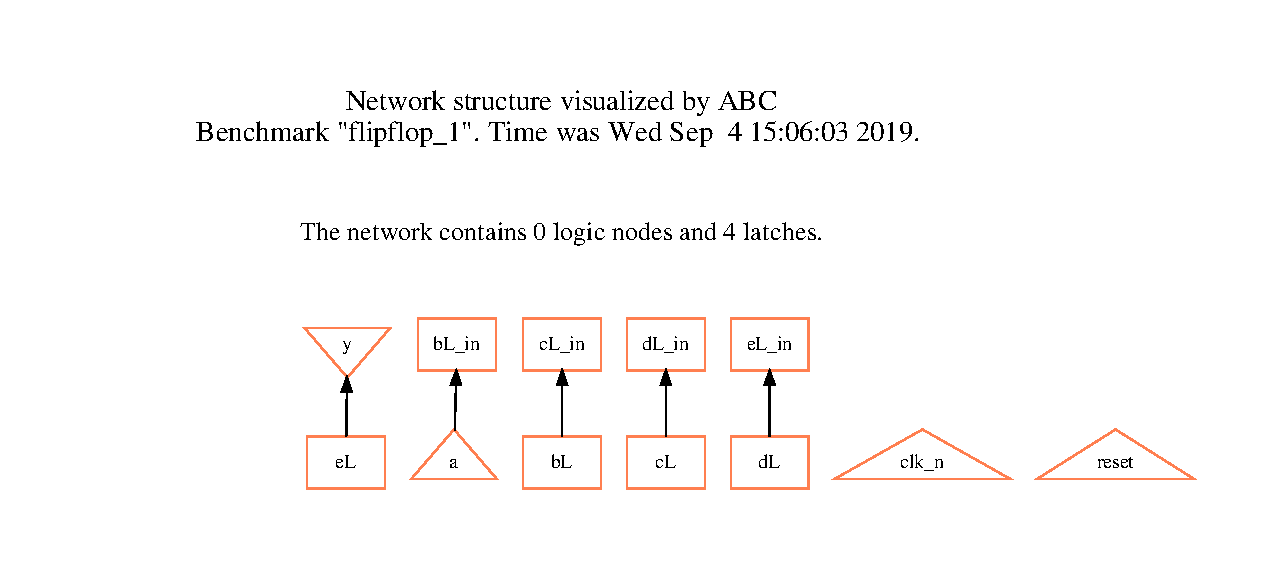
\includegraphics[width=15cm]{MScThesisTemplate/Figs/xsim.pdf}
    \caption{\footnotesize xsim}
\end{figure}
\renewcommand{\baselinestretch}{1.5}
\chapter{Measurement}
\label{App:measurement}
\begin{table}[htbp]
    \centering
    \begin{tabular}{c|c|c|c|c}
    \hline
        Num & $1^{st}$ &$2^{nd}$ &$3^{rd}$ &ave\\
        \hline
        1 &  10.3625& 10.5777&	11.5796&	10.83993333\\
        10 &34.9239&	36.3843	&37.9927&	36.43363333\\
        100 &41.1955&	55.1316	&52.8391&	49.72206667\\
        1000 &90.4534&	77.4710&	83.1347	&83.68636667\\
        10000 &728.1557&	431.0128&	504.4528&	554.5404333\\
        100000 & 4055.7796	&4051.6156&	4889.3483&	4332.247833\\
    \end{tabular}
    \caption{\footnotesize Data of \texttt{general.v}}
    \label{tab:d_g}
\end{table}

\begin{table}[htbp]
    \centering
    \begin{tabular}{c|c|c|c|c}
    \hline
        Num & $1^{st}$ &$2^{nd}$ &$3^{rd}$ &ave\\
        \hline
        1 &  11.606&	10.8229	&11.1331&	11.18733333\\
        10 &22.5682&	34.9506	&35.3318&	30.9502\\
        100 &50.1338&	46.3471	&50.4967&	48.99253333\\
        1000 &159.5571&	138.0580&	134.7428&	144.1193\\
        10000 &863.4109	&847.9672&	826.1776&	845.8519\\
        100000 & 7321.337&	8232.4844&	8216.6564&	7923.4926\\
    \end{tabular}
    \caption{\footnotesize Data of \texttt{embedded.v}}
\end{table}
\begin{table}[htbp]
    \centering
    \begin{tabular}{c|c|c|c|c}
    \hline
        Num & $1^{st}$ &$2^{nd}$ &$3^{rd}$ &ave\\
        \hline
        1 &  11.0318&	10.1481	&10.5002&	10.56003333\\
        10 &12.7669	&12.2207&	11.8063&	12.264633333\\
        100 &23.1209&	26.9675	&27.1547&	25.7477\\
        1000 &65.0746&	63.6028	&71.4553&	66.7109\\
        10000 &314.1	&310.2118&	287.1644&	303.8254\\
        100000 & 2726.7935&	2941.2117&	2901.7128&	2856.572667\\
    \end{tabular}
    \caption{\footnotesize Data of \texttt{flipflop.v}}
\end{table}
\begin{table}[htbp]
    \centering
    \begin{tabular}{c|c|c|c|c}
    \hline
        Num & $1^{st}$ &$2^{nd}$ &$3^{rd}$ &ave\\
        \hline
        1 &  10.8444&	10.3499	&9.7557	&10.31666667\\
        10 &13.9057&	13.8499&	13.1431	&13.6329\\
        100 &29.5568&	29.8336&	34.8811	&31.42383333\\
        1000 &85.1189&	70.2971&	96.4864	&83.96746667\\
        10000 &306.1257	&386.8924&	335.2358&	342.7513\\
        100000 & 3303.2233&	3401.7683&	3326.8053&	3343.9323\\
    \end{tabular}
    \caption{\footnotesize Data of \texttt{FSM.v}}
\end{table}

\begin{table}[htbp]
    \centering
    \begin{tabular}{c|c|c|c|c}
    \hline
        Num & 10 &100&1000&10000\\
        \hline
        $check\_abc.sh$&0.3954 &3.85&37.3858&364.855\\
       $check\_abs_sis.sh$ &0.2710&2.9800&30.4020&297.8260\\
    \end{tabular}
    \caption{\footnotesize Data of \texttt{script execution.v}}
\end{table}

\begin{table}[htbp]
    \centering
    \begin{tabular}{c|c|c|c|c}
    \hline
        Num & $1^{st}$ &$2^{nd}$ &$3^{rd}$ &ave\\
        \hline
        2 &  0.339&	0.3380&	0.326&	0.334333333\\
        4 &0.394&	0.3930&	0.372&	0.386333333
\\
        6 &0.422&	0.4650	&0.469&	0.452
\\
        8 &0.532&	0.5290&	0.509&	0.523333333
\\
        10 &0.577&	0.5780&	0.58&	0.578333333
\\
    \end{tabular}
    \caption{\footnotesize Data of NumPort analysis}
\end{table}

\begin{table}[htbp]
    \centering
    \begin{tabular}{c|c|c|c|c}
    \hline
        Num & $1^{st}$ &$2^{nd}$ &$3^{rd}$ &ave\\
        \hline
        2 &  0.528&	0.5200&	0.518&	0.522
\\
        4 &0.613&	0.7010&	0.672&	0.662

\\
        6 &0.693&	0.7010&	0.72&	0.704666667

\\
        8 &0.739&	0.7200&	0.745&	0.734666667

\\
        10 &0.874&	0.8440&	0.828&	0.848666667

\\
    \end{tabular}
    \caption{\footnotesize Data of NumSubmodule analysis}
\end{table}

%%%%%%%%%%%%%%%%%%%%%%%%%%%%%%
% The end of a LaTeX document
\end{document}

%%%%%%%%%%The END%%%%%%%%%%%%%%%%%%%% 